%%----------------------------------------------------------------------
%%----------------------------------------------------------------------
\missiontitle{Mission 1: Ambush}

%\teaser{Recon forces desperately searching for weaknesses in the enemy
%  lines collide!}

This is an asymmetric mission; players alternate games as the
\textbf{Attacker} and the \textbf{Defender}.

%%----------------------------------------------
  \begin{columns}
\begin{tablesetup}    
  There is no roll-off for deployment zones or order.  The Defender
  begins by choosing their player table edge and a diagonal line
  between two opposing corners of the board.  Place a primary
  objective marker at table center, and two more each 12''x12'' from
  those table corners.  The Defender then deploys their models inside
  their deployment zone: Anywhere wholely within 6'' of the chosen
  diagonal.

  Next the Attacker deploys anywhere on the board, but each model must
  be at least 18'' from every Defender model if not in line-of-sight
  of any Defender model, and at least 24'' from every Defender model
  if in line-of-sight of any Defender model.  The Attacker's player
  table edge is that opposite the Defender's.
\end{tablesetup}

\bigskip
\missionheading{Mission Specific Rules}
\vspace{-0.5em}
\nightfighting

\vfill\vbox to 0pt{}
\columnbreak
\bigskip\centerline{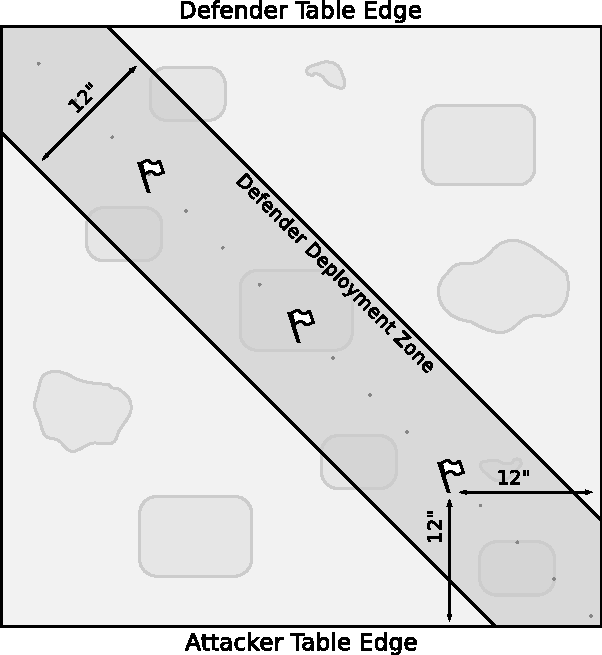
\includegraphics[width=\linewidth]{maps/mission1.pdf}}
  \end{columns}
\vspace{-2.5em}

%%----------------------------------------------
%\begin{missionrules}

\missionsubheading{Hasty Redoubts.} During deployment the Defender may
designate~3 distinct pieces of terrain at least partially in their
deployment zone.  Cover saves granted by that terrain are improved
by~1, to no better than~3+.

\missionsubheading{Sneak Attack.} During deployment the Attacker may
grant the Outflank special rule to up to~3 of their units (embarked
units do not count). After all deployment concludes, the Attacker
chooses to play first or second.

  % Defender units at least partially
  % within 3'' of the primary objective markers \emph{may} re-roll
  % failed morale checks.

%\end{missionrules}


%%----------------------------------------------
\begin{scoring}
  
\begin{primaries}

  Before any Scout redeployments, both players secretly choose one of
  the following primary scoring mechanisms for themselves:

  \begin{itemize}
  \item {\textit{Continuous.}} Beginning with Turn~2, score~1 victory
    point at the end of each of your player turns for each primary
    objective marker you control.

  \item {\textit{End Game.}} At game end, score~3 victory points for
    each primary objective marker you control.

  \end{itemize}
  This selection is declared along with the choice of secondary
  objective, below.  Remember that \underline{no more than}
  \underline{9 victory points may be earned toward primary
    objectives}.

\end{primaries}

\end{scoring}
